\documentclass[11pt, english]{article}
\usepackage{graphicx}
\usepackage[colorlinks=true, linkcolor=blue]{hyperref}
\usepackage[russian,english]{babel}
\selectlanguage{russian}
\usepackage[utf8]{inputenc}
\usepackage[svgnames]{xcolor}
\usepackage{amsmath}

\usepackage{listings}
\usepackage{afterpage}
\pagestyle{plain}

\definecolor{dkgreen}{rgb}{0,0.6,0}
\definecolor{gray}{rgb}{0.5,0.5,0.5}
\definecolor{mauve}{rgb}{0.58,0,0.82}

% \lstset{language=R,
%     basicstyle=\small\ttfamily,
%   stringstyle=\color{DarkGreen},
%     otherkeywords={0,1,2,3,4,5,6,7,8,9},
%     morekeywords={TRUE,FALSE},
%     deletekeywords={data,frame,length,as,character},
%     keywordstyle=\color{blue},
%     commentstyle=\color{DarkGreen},
% }

\lstset{frame=tb,
language=java,
aboveskip=3mm,
belowskip=3mm,
showstringspaces=false,
columns=flexible,
numbers=none,
keywordstyle=\color{blue},
numberstyle=\tiny\color{gray},
commentstyle=\color{dkgreen},
stringstyle=\color{mauve},
breaklines=true,
breakatwhitespace=true,
tabsize=3
}

\usepackage{here}


\textheight=21cm
\textwidth=17cm
%\topmargin=-1cm
\oddsidemargin=0cm
\parindent=0mm
\pagestyle{plain}

%%%%%%%%%%%%%%%%%%%%%%%%%%
% La siguiente instrucción pone el curso automáticamente%
%%%%%%%%%%%%%%%%%%%%%%%%%%

\usepackage{color}
\usepackage{ragged2e}
\usepackage[T1]{fontenc}

\global\let\date\relax
\newcounter{unomenos}
\setcounter{unomenos}{\number\year}
\addtocounter{unomenos}{-1}
\stepcounter{unomenos}
\gdef\@date{\arabic{unomenos}}

\begin{document}

    \begin{titlepage}

        \begin{center}
            \vspace*{-1in}
            \begin{figure}[htb]
                \begin{center}
                    
\includegraphics[width=8cm]{bw_w_rus.png}
                \end{center}
            \end{figure}

            Факультет Программной Инженерии и Компьютерных Технологий \\
            \vspace*{0.15in}
            Вычислительная математика \\
            \vspace*{0.4in}
            \begin{large}
                ЛАБОРАТОРНАЯ РАБОТА №5\\
            \end{large}
            \vspace*{0.2in}
            \begin{Large}
                \textbf{Решение ОДУ} \\
            \end{Large}
            \vspace*{0.3in}
            \begin{large}
                Усовершенствованный метод Эйлера \\
            \end{large}
            \vspace*{0.3in}
            \rule{80mm}{0.1mm}\\
            \vspace*{0.1in}
            \begin{large}
                Преподаватель: Перл О.В. \\
                Выполнил: Куприянов А.А, P3212 \\
            \end{large}
            \vspace*{3.6in}

            Санкт-Петербург \\
            2020
        \end{center}
    \end{titlepage}

    \newcommand{\CC}{C\nolinebreak\hspace{-.05em}\raisebox{.4ex}{\tiny\bf +}\nolinebreak\hspace{-.10em}\raisebox{.4ex}{\tiny\bf +}}
    \def\CC{{C\nolinebreak[4]\hspace{-.05em}\raisebox{.4ex}{\tiny\bf ++}}}

    \tableofcontents
    \newpage


    \section{Теория}
    Для того чтобы лучше понять усовершенствованный метод Эйлера, следует понять как работает его исходная версия

    \subsection{Метод Эйлера}
    \begin{center}
        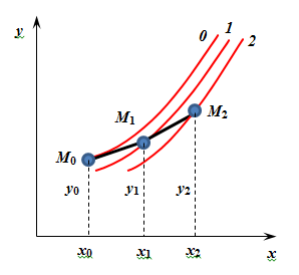
\includegraphics[width=7cm]{euler-1.png}
    \end{center}
    Если уравнение $$y^{'} = f(x, y) ,\: y(x_0) = y_0$$ не может быть решена аналитически, то нужно прибегнуть к численным методам для получения приближений к решению уравнения.\\

    Мы можем вычислить приближенные значения в равноотстоящих точках $x_0, x_1, ..., x_n = b$ в интервале $[x_0, b]$, так что:
    $$x_i = x_0 + ih, \: i = 0,1,...,n$$
    где
    $$h = \frac{b - x_0}{n}$$

    Одним из методов позволяющих сделать это, является метод Эйлера\\

    Тем не менее, это очень грубый метод, который редко используется на практике. Скорее, его используют для иллюистративных целей из-за его простоты.\\

    Метод Эйлера основан на предположении, что касательная к интегральной кривой уравнения в $(x_i, y(x_i))$ апроксимирует интегральную кривую на отрезке $[x_i, x_{i+1}]$\\

    Так как наклон интегральной кривой уравнения в точке $(x_i, y(x_i))$ равен $y(x_i)^{'} = f(x_i, y(x_i))$, уравнение касательной кривой в точке $(x_i, y(x_i))$ является:
    $$y = y(x_i) + f(x_i, y(x_i))(x - x_i)$$

    Пологая, что $x = x_{i + 1} = x_i + h$, получим:
    $$y_{i + 1} = y(x_i) + hf(x_i, y(x_i))$$
    как апроксимацию для значения $y(x_{i + 1})$

    И так как мы знаем начальное условие $y(x_0) = y_0$ мы можем использовать это уравнение с $i = 0$ для вычисления
    $$y_1 = y_0 + hf(x0, y0)$$
    Также и для $y2$, но следует заметить, что мы не можем вычислить $y2$ пока не вычислим $y1$. \\

    Общий алгоритм Эйлера начинается с известного значения $y(x_O) = y_0$ и вычисления $y_1, y_2, ... , y_n$
    $$y_{i+1} = y_i + hf(x_i, y_i),\: 0 \leq i \leq n - 1$$

    \subsection{Усовершенствованный метод Эйлера}

    В методе Эйлера ошибка усечения равна $O(h)$.
    Можно предположить, что мы можем достичь высокой точности, просто выбрав достаточно маленький размер шага. \\

    Но это не совсем так. Во-первых, чем меньше мы делаем шаг, тем больше ошибка округления (так как вычисления происходят на машинах, то присутствует машинный эпсилон, например). Во-вторых, вычисление $f(x,y)$ является довольно дорогим, поэтому мы не можем позволить себе слишком маленькие шаги. \\

    Основным отличием усовершенствованного метода Эйлера является то, что при апроксимировании интегральной кривой в точке $(x_i, y(x_i))$ используется линия проходящая через $(x_i, y(x_i))$ с наклоном
    $$m_i = \frac{f(x_i, y(x_i)) + f(x_{i+1}, y(x_{i+1}))}{2}$$

    Тогда уравнение апроксимирующей линии превращается в
    $$y = y(x_i) + \frac{f(x_i, y(x_i)) + f(x_{i+1}, y(x_{i+1}))}{2} (x - x_i)$$

    Положив $x = x_{i+1} = x_i + h$ получим:
    $$y_{i+1} = y(x_i) + \frac{h}{2}(f(x_i, y(x_i)) + f(x_{i+1}, y(x_{i+1})))$$
    для апроксимации $y(x_{i+1})$ \\

    Мы уже знаем значение $y(x_i)$, но не значение $y(x_{i+1})$.
    Поэтому полученная схема является неявной.
    В этом случае мы можем заменить $y(x_{i+1})$ на $y_i + hf(x_i, y_i)$ из метода Эйлера. \\

    Тогда получим итоговую формулу:
    \[y_{i+1} = y_i + \frac{h}{2}(f(x_i, y(x_i)) + f(x_{i+1}, y_i + hf(x_i, y_i)))\]

    Сравним апроксимацию к $e$ этих двух методов:
    \begin{center}
        \begin{tabular}{||c | c | c | c||}
            \hline
            n & метод Эйлера & Усовершенствованный метод Эйлера & Точное значение \\ [0.5ex]
            \hline\hline
            12 & 2.613035290 & 2.707188994 & 2.718281828 \\
            \hline
            24 & 2.663731258 & 2.715327371 & 2.718281828 \\
            \hline
            48 & 2.690496599 & 2.717519565 & 2.718281828 \\
            \hline
        \end{tabular}
    \end{center}
    \newpage


    \section{Реализация}

    \subsection{Блок-схема}
    \begin{center}
        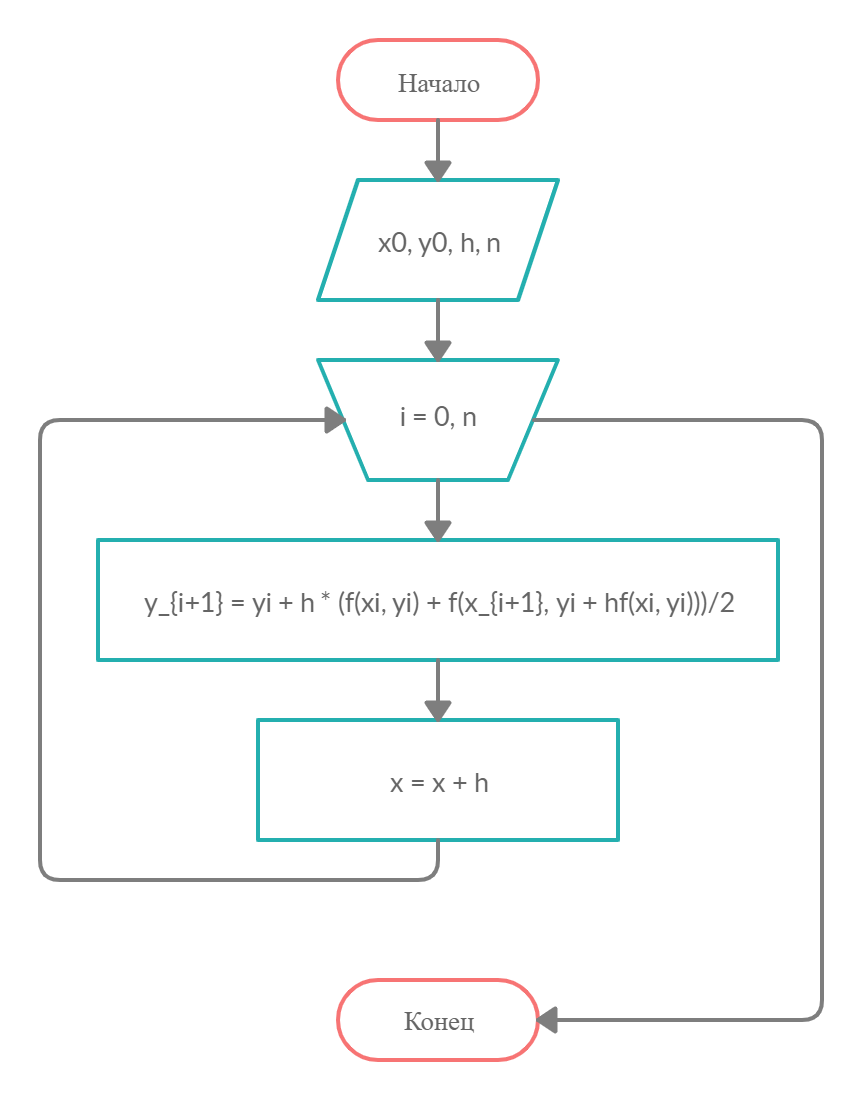
\includegraphics[width=8cm]{schema.png}
    \end{center}

    \newpage

    \subsection{Программа на Java}
    \begin{lstlisting}
@Override
public List<Dot> solve(DiffEquation equation, double x0, double y0, double accuracy) {
        EulerSolverConfig config = calculateConfiguration(equation, x0, y0, accuracy);
        return solve(equation, x0, y0, config.pointsAmount, config.step);
}

@Override
public List<Dot> solve(DiffEquation equation, double x0, double y0, int pointsAmount, double step) {
        List<Dot> dots = new ArrayList<>();
        dots.add(new SimpleDot(x0, y0));

        double x = x0;
        double calculatedY = y0;

        for (int i = 0; i < pointsAmount; i++) {
        double approximatedY = approximateNextY(equation, step, x, calculatedY);
            calculatedY = calculateY(equation, step, x, calculatedY, approximatedY);
            x += step;
            dots.add(new SimpleDot(x, calculatedY));
}

        return dots;
}

private double approximateNextY(DiffEquation equation, double h, double x, double y){
        return y +  h * equation.apply(x, y);
}

private double calculateY(DiffEquation equation, double h, double x, double y, double approximatedY){
        return y +  h * (equation.apply(x, y) + equation.apply(x +  h, approximatedY)) / 2;
}

    \end{lstlisting}
    \newpage


    \section{Результаты работы программы}
    Эксперименты проводились на нескольких функциях
    \begin{itemize}
        \item $y' = y$
        \item $y' = sin(x)$
        \item $y' = y( 2sin(x) + 1)$
    \end{itemize}

    \subsection{$y' = y$}
    Общее решение уравнения имеет вид $y(x) = c_1 e^x$ \\
    Для задачи Коши используем несколько параметров и вычислим значение в $x=0$
    \begin{center}
        \resizebox{\columnwidth}{!}{%
            \begin{tabular}{|c | c | c | c |}
                \hline
                Начальные условия & Решение задачи & Точное значение & Интеролированное значение\\ [0.5ex]
                \hline
                $y(0.8) = -0.8 $ & $y(x) = -0.359463e^x$ & -0.359463 & -0.359493 \\
                \hline
                $y(1) = 1$ & $y(x) = e^{x-1}$ & 0,367879 & 0.367918\\
                \hline
                $y(0.1) = -0.1$ & $y(x) = -0.0904837e^x$ & -0.090483 & -0.090484\\
                \hline
            \end{tabular}
        }
    \end{center}

    \subsection{$y' = sin(x)$}
    Общее решение уравнения имеет вид $y(x) = c_1 - cos(X)$ \\
    Для задачи Коши используем несколько параметров и вычислим значение в $x=0$
    \begin{center}
        \resizebox{\columnwidth}{!}{
            \begin{tabular}{|c | c | c | c |}
                \hline
                Начальные условия & Решение задачи & Точное значение & Интеролированное значение\\ [0.5ex]
                \hline
                $y(0.8) = -0.8 $ & $y(x) = -cos(x) - 0.103293$ & -1.103293 & -1.103277 \\
                \hline
                $y(1) = 1$ & $y(x) = -cos(x) + 1 + cos(1)$ & 0.540302 & 0.540326\\
                \hline
                $y(0.1) = -0.1$ & $y(x) = 0.895004 - cos(x)$ & -0.104996 & -0.104995\\
                \hline
            \end{tabular}
        }
    \end{center}

    \subsection{$y' = y(2sin(x) + 1)$}
    Общее решение уравнения имеет вид $y(x) = c_1 e^{(x - 2 cos(x))}$ \\
    Для задачи Коши используем несколько параметров и вычислим значение в $x=0$
    \begin{center}
        \resizebox{\columnwidth}{!}{
            \begin{tabular}{|c | c | c | c |}
                \hline
                Начальные условия & Решение задачи & Точное значение & Интеролированное значение\\ [0.5ex]
                \hline
                $y(0.8) = -0.8 $ & $y(x) = -1.44813 e^{(x - 2 cos(x))}$ & -0.195983 & -0.196010 \\
                \hline
                $y(1) = 1$ & $y(x) = e^{(x - 2 cos(x) - 1 + 2 cos(1))}$ & 0.146695 & 0.146730\\
                \hline
                $y(0.1) = -0.1$ & $y(x) = -0.661942 e^{(x - 2 cos(x))}$ & -0.089584 & -0.089606\\
                \hline
            \end{tabular}
        }
    \end{center}


    \newpage


    \section{Вывод}
    Численные методы могут оказать помощь в тех случаях, когда не работает аналитический подход. Тогда мы можем применить один из численных методов для приближенного решения.
    \newline\newline
    Тем не менее, возникает два вида погрешностей в виду особенности среды исполнения и самих методов. Ошибка усечения является погрешностью самого метода, ведь, например, в методах Эйлера для решения ОДУ мы апроксимируем некоторые значения из-за чего возникает погрешность. Также есть ошибка округления связанная с машинными операциями.
    \newline\newline
    Основываясь на них мы можем проводить оценку численных методов и выбрать наиболее подходящий из них.
    \newline\newline
    Например, сравнивая метод Эйлера и усовершенствованный метод Эйлера мы можем выяснить, что несмотря на то, что мы можем получить сколь угодно хорошую точность уменьшая шаг - мы упираемся в характеристики вычислительной машины.
    \newline\newline
    Усовершенствованный метод Эйлера при сравнении с другими одношаговыми методами оказался точнее, чем обычный метод Эйлера, но менее точным, чем метод Рунге-Кутта (метод Рунге-Кутты 4 порядка), хотя в методе Эйлера выполняется меньше операций.
    \newline\newline
    Также сравнивая с многошаговыми методами, то с помощью метода Эйлера мы сразу можем начать счет по одному лишь известному значению $y_0$. Кроме того, например,метод Адамса не позволяет (без усложнения формул) изменить шаг в процессе счета. Такого недостатка нету в одношаговых методах

\end{document}